\chapter{L'esperimento CRESST}
\label{ch:CRESST}

L'esperimento CRESST (Cryogenic Rare Event Search with Superconducting Thermometers) è una collaborazione internazionale finalizzata alla ricerca diretta di WIMPs nella regione delle basse masse ($ \leq 1 \text{ GeV}$). L'apparato sperimentale è situato presso i Laboratori Nazionali del Gran Sasso (LNGS) dell'INFN in Italia.
La collocazione sotto 1400 metri di roccia permette di schermare efficacemente il flusso di muoni cosmici.

Per identificare i rari e infinitesimi depositi di energia rilasciati dall'interazione delle WIMP con i nuclei del bersaglio, CRESST impiega rivelatori criogenici a stato solido portati a temperature dell'ordine dei millikelvin (10 mK), prossime allo zero assoluto. Tramite questo processo, che permette di ridurre al minimo il rumore termico di fondo, diventa possibile misurare i minuscoli innalzamenti di temperatura causati dai rinculi nucleari e spingere la soglia di rivelazione energetica a livelli tra i più bassi al mondo, aprendo una finestra osservativa cruciale sulla materia oscura di massa leggera.

\section{Il principio di rivelazione: il doppio canale}
\label{sec:doppio_canale}

Il cuore tecnologico dell'esperimento CRESST risiede nell'utilizzo di target cristallini scintillanti operati come calorimetri criogenici a bassissima temperatura. La scelta del materiale riflette la necessità di massimizzare la sezione d'urto di interazione con le WIMP (\ref{subsec:rate_sezionedurto}) e, al contempo, di disporre di un eccellente mezzo di scintillazione; per queste ragioni, i moduli rivelatori standard di CRESST-III impiegano cristalli di tungstato di calcio ($\text{CaWO}_4$). 

Quando una particella (sia essa una WIMP del segnale o una particella del fondo ambientale) attraversa il cristallo bersaglio, interagisce con la materia depositando una determinata energia $E_{\text{dep}}$. Questo rilascio di energia si propaga nel mezzo dando origine a due processi fisici distinti, che costituiscono i due canali di lettura indipendenti dell'esperimento:

\begin{enumerate}
    \item \textbf{Il canale fononico (calore):} La quasi totalità dell'energia depositata ($>99\%$) viene convertita in vibrazioni reticolari del cristallo, ovvero in fononi non termici. Questi fononi si propagano nel materiale fino a raggiungere la superficie del cristallo, dove un sensore termico ne misura l'innalzamento di temperatura complessivo. Poiché la frazione di energia convertita in calore è pressoché indipendente dal tipo di particella interagente, il canale fononico fornisce una misura precisa e diretta dell'energia depositata, secondo la relazione:
    \begin{equation}
        \Delta T = \frac{E_{\text{dep}}}{C}
    \end{equation}
    dove $C$ è la capacità termica del cristallo bersaglio. A parità di energia depositata, disporre di una capacità termica estremamente bassa permette di massimizzare l'ampiezza del segnale termico $\Delta T$. Per questa ragione i cristalli sono mantenuti a temperature criogeniche dell'ordine del millikelvin, regime in cui la capacità termica segue la legge di Debye ($C \propto T^3$) e risulta drasticamente ridotta rispetto ai valori a temperatura ambiente.
    
    \item \textbf{Il canale fotonico (luce):} Una piccola frazione dell'energia depositata (tipicamente l'1\% o meno) viene emessa sotto forma di fotoni di scintillazione. Per raccogliere questa luce, ogni cristallo di $\text{CaWO}_4$ è accoppiato a un rivelatore di luce indipendente posto nelle immediate vicinanze. La quantità di luce prodotta è fortemente dipendente dalla densità di ionizzazione della particella incidente e, di conseguenza, dalla sua natura (rinculo elettronico dovuto a particelle $\beta/\gamma$ oppure rinculo nucleare dovuto a neutroni, WIMP o particelle $\alpha$).
\end{enumerate}

L'adozione di questa tecnica a doppio canale è l'elemento chiave che conferisce a CRESST la sua straordinaria sensibilità nella ricerca di eventi rari. Mentre il canale fononico determina con precisione l'energia dell'evento e definisce la soglia minima di rivelazione dell'esperimento, il canale fotonico fornisce l'informazione cruciale per identificare la natura dell'interazione. La correlazione tra l'energia misurata sotto forma di calore e quella raccolta sotto forma di luce permette infatti di definire una variabile discriminante fondamentale, il \textit{Light Yield}, di cui si discuterà nel dettaglio nella Sezione~\ref{sec:light_yield}.

\section{Come viene letto il segnale: TES e SQUID}
\label{sec:tes_squid}

La straordinaria sensibilità energetica dell'esperimento CRESST, capace di registrare innalzamenti di temperatura microscopici nei cristalli di $\text{CaWO}_4$, richiede una tecnologia di lettura all'avanguardia. Il sistema di sensoristica si basa sulla combinazione di due dispositivi a superconduzione operanti in sinergia: il \textit{Transition Edge Sensor} (TES), che funge da termometro ad altissima risoluzione, e il \textit{Superconducting Quantum Interference Device} (SQUID), utilizzato come amplificatore di corrente a bassissimo rumore.

\subsubsection{Il Transition Edge Sensor (TES)}

Il TES è un termometro criogenico costituito da una sottile striscia di materiale superconduttore (tipicamente tungsteno) depositato direttamente sulla superficie del cristallo bersaglio e del rivelatore di luce. Il principio di funzionamento sfrutta l'estrema dipendenza della resistenza elettrica dalla temperatura nella stretta regione di transizione tra lo stato normale e lo stato superconduttore.

Mantenendo il sistema a una temperatura di lavoro $T_0$ stabilizzata esattamente al centro di questa curva di transizione, il TES presenta una resistenza parziale. Quando un fonone generato nel cristallo lo colpisce, cede la sua energia causando un microscopico incremento di temperatura $\Delta T$. Poiché la curva della resistenza del TES è estremamente ripida in questa regione, anche un aumento di temperatura dell'ordine di pochi millikelvin provoca un cambiamento significativo della resistenza $\Delta R$ del sensore, come illustrato in Figura \ref{fig:tes_curve}.
\begin{figure}
    \centering
    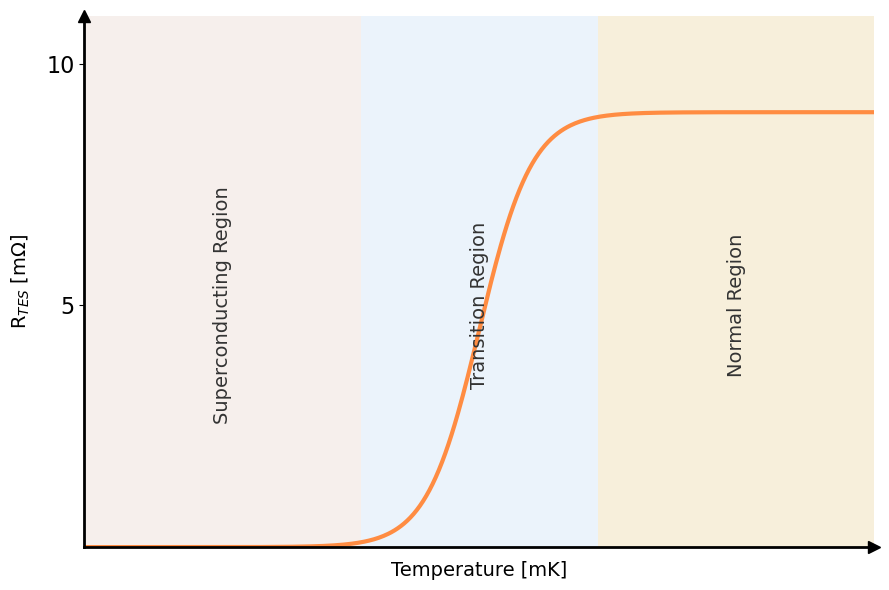
\includegraphics[width=0.7\textwidth]{figures/curva_transizione.png}
    \caption{Curva di transizione del TES. La resistenza passa rapidamente dallo stato superconduttore (R=0) allo stato normale (R=R$_n$) in un intervallo di temperatura molto ristretto.}
    \label{fig:tes_curve}
\end{figure}

Un secondo TES è posizionato sopra il light detector. Non potendo usare tubi fotomoltiplicatori per la rivelazione della luce, che introdurrebbero una quantità di radioattività intrinseca inaccettabile, nelle immediate vicinanze del cristallo di $\text{CaWO}_4$ viene posizionato un disco sottilissimo di silicio (il light detector), che funge da rivelatore di luce. I fotoni di scintillazione prodotti nel cristallo vengono assorbiti dal disco, generando fononi non termici che vengono rilevati dal TES sovrastante. L'apparato sperimentale è illustrato in figura \ref{fig:detector_module}.
\begin{figure}
    \centering
    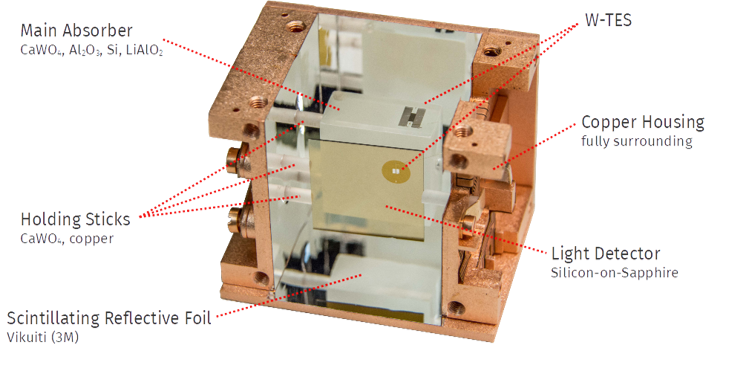
\includegraphics[width=0.7\textwidth]{figures/Detector_simple.png}
    \caption{Schema di un modulo rivelatore CRESST. Immagine tratta da \cite{cresst_detectors_2026}.}
    \label{fig:detector_module}
\end{figure}

Quando il cristallo viene colpito da una particella, il TES si scalda in tempi dell'ordine del millisecondo. Per poter registrare un evento successivo è necessario attendere che il sensore si raffreddi e torni alle condizioni di lavoro iniziali, un processo che avviene tipicamente in qualche decina di millisecondi (10-50~ms). Questo rapido ritorno all'equilibrio è possibile poiché all'aumentare della temperatura del TES, la sua resistenza elettrica subisce un brusco incremento che fa diminuire la corrente. Di conseguenza, la potenza dissipata per effetto Joule ($P = V^2/R$) si riduce, accelerandone il raffreddamento.

\subsubsection{Lo SQUID}

La variazione di corrente $\Delta I$ indotta nel TES dal passaggio di una particella è un segnale infinitesimo, dell'ordine dei nanoampere, che non potrebbe essere trasportato fino all'elettronica a temperatura ambiente tramite cavi convenzionali senza essere completamente sommerso dal rumore termico e dalle interferenze. Per ovviare a questo problema, la catena di lettura di CRESST introduce lo SQUID (\textit{Superconducting Quantum Interference Device}).


Come illustrato nello schema di Figura~\ref{fig:squid_circuit}, il circuito di bias del TES è connesso in parallelo ad un'induttanza. Quando un evento termico nel cristallo fa crescere la resistenza del TES, una maggior quantità di corrente viene deviata verso l'induttanza. Questa corrente genera un campo magnetico proporzionale che concatena l'anello dello SQUID.

\begin{figure}[htbp]
    \centering
    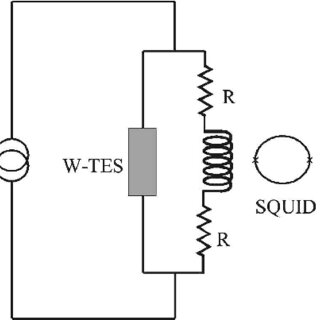
\includegraphics[width=0.45\textwidth]{figures/Readout-circuit-for-the-superconducting-thermometer-TES_Q320.jpg}
    \caption{Schema elettrico semplificato del circuito di lettura. La variazione di resistenza del TES modifica la ripartizione della corrente, che si traduce in un campo magnetico che concatena l'anello dello SQUID.}
    \label{fig:squid_circuit}
\end{figure}

Lo SQUID converte questo infinitesimo flusso magnetico in una variazione di tensione elettrica ($\Delta V$) misurabile dall'elettronica a temperatura ambiente. Offrendo un guadagno eccezionale e un rumore intrinseco virtualmente nullo, questo sistema permette di preservare e digitalizzare l'informazione sul rilascio energetico originario anche per eventi estremamente deboli, inferiori al $\text{keV}$.

\subsection{Il sistema di refrigerazione: il criostato a diluizione}
\label{subsec:criostato}

Per mantenere i moduli rivelatori, i TES e gli SQUID alla temperatura di lavoro millikelvin ($10\text{ mK}$) richiesta dall'esperimento, è necessario un sistema di refrigerazione sofisticato, capace di abbattere la temperatura di oltre cinque ordini di grandezza rispetto all'ambiente esterno. Questo compito è affidato a un criostato a diluizione di idrossido di elio ($^3\text{He}/^4\text{He}$), che opera attraverso una serie di stadi di raffreddamento progressivi:

\begin{enumerate}
    \item \textbf{Primo stadio (Pre-raffreddamento a $\sim 77\text{ K}$):} Il primo abbattimento termico massivo sfrutta il potere refrigerante dell'azoto liquido. Questo stadio riduce la temperatura del nucleo interno del criostato da temperatura ambiente fino a circa $77\text{ K}$ (temperatura di ebollizione dell'azoto), fungendo al contempo da prima barriera termica contro l'irraggiamento esterno.
    
    \item \textbf{Secondo stadio (Fase dell'Elio liquido a $\sim 4.2\text{ K}$ e $\sim 1\text{ K}$):} Il sistema viene successivamente raffreddato sfruttando le proprietà termiche dell'Elio liquido ($^4\text{He}$). A pressione atmosferica, l'elio bolle a $4.2\text{ K}$. Attraverso un sofisticato sistema di vuoto forzato è possibile abbassare ulteriormente la temperatura di ebollizione, spingendo questo stadio fino a circa $1\text{ K}$.
    
    \item \textbf{Terzo stadio (Unità a diluizione a $\sim 10\text{ mK}$):} Per scendere sotto la barriera di $1\text{ K}$ è necessario sfruttare le proprietà termodinamiche della miscela di due isotopi stabili dell'elio: l'Elio-3 ($^3\text{He}$) e l'Elio-4 ($^4\text{He}$). Quando questa miscela viene raffreddata sotto gli $0.8\text{ K}$, essa subisce una separazione spontanea in due fasi distinte: una fase "ricca" di $^3\text{He}$ (più leggera, che galleggia sopra) e una fase "diluita" (costituita quasi interamente da $^4\text{He}$ superfluido, in cui è disciolta una piccola frazione di $^3\text{He}$). 
\end{enumerate}

Tramite un sistema di pompaggio, gli atomi di $^3\text{He}$ vengono forzati ad attraversare la linea di separazione, passando dalla fase ricca alla fase diluita. Questo processo è endotermico: l'attraversamento della barriera richiede energia, che viene sottratta direttamente dall'ambiente circostante sotto forma di calore. È proprio grazie a questo continuo passaggio di fase quantistico che il criostato riesce ad assorbire il calore residuo dei rivelatori e a stabilizzare stabilmente l'intero apparato sperimentale alla temperatura criogenica di $10\text{ mK}$. Poiché questo meccanismo di raffreddamento utilizza materiali non radiopuri (serbatoi per l'azoto e l'elio, valvole e saldature etc...), il criostato deve stare al di fuori del modulo rivelatore. La temperatura criogenica è trasmessa al modulo tramite un collegamento in rame ultrapuro, che funge da ponte termico tra il criostato e il rivelatore come mostrato in Figura \ref{fig:shielding}.

\subsection{Discriminazione del fondo: il Light Yield}
\label{sec:light_yield}

Come introdotto nel paragrafo \ref{sec:doppio_canale} l'utilizzo di una tecnica a doppio canale (calore e luce) permette non solo di determinare l'energia totale rilasciata in un evento, ma anche di identificare la natura della particella interagente. Il parametro fondamentale per operare questa selezione dei dati è il \textit{Light Yield} ($LY$), definito come il rapporto tra l'energia misurata nel canale fotonico ($E_{\text{luce}}$) e l'energia totale depositata nel canale fononico ($E_{\text{calore}}$):

\begin{equation}
    LY = \frac{E_{\text{luce}}}{E_{\text{calore}}}
\end{equation}

La fisica alla base della discriminazione risiede nel fenomeno del \textit{quenching} della scintillazione: particelle ad alta densità di ionizzazione (come i nuclei di rinculo) perdono una frazione maggiore di energia in canali non radiativi rispetto a particelle a bassa densità di ionizzazione (come elettroni e fotoni). Di conseguenza, a parità di energia termica depositata nel cristallo ($E_{\text{calore}}$), un rinculo nucleare produrrà una quantità di luce significativamente inferiore rispetto a un rinculo elettronico, posizionandosi a valori di $LY$ decisamente più bassi.

Nel caso specifico dei cristalli di $\text{CaWO}_4$ impiegati in CRESST, il target è composto da tre diversi nuclei bersaglio (Calcio, Ossigeno e Tungsteno), ciascuno caratterizzato da un differente fattore di quenching dovuto alla diversa massa nucleare. Questa particolarità si traduce nella separazione dei dati in bande ben distinte all'interno del piano $LY$ in funzione dell'energia, come illustrato nella Figura~\ref{fig:bands}.

\begin{figure}[htbp]
    \centering
    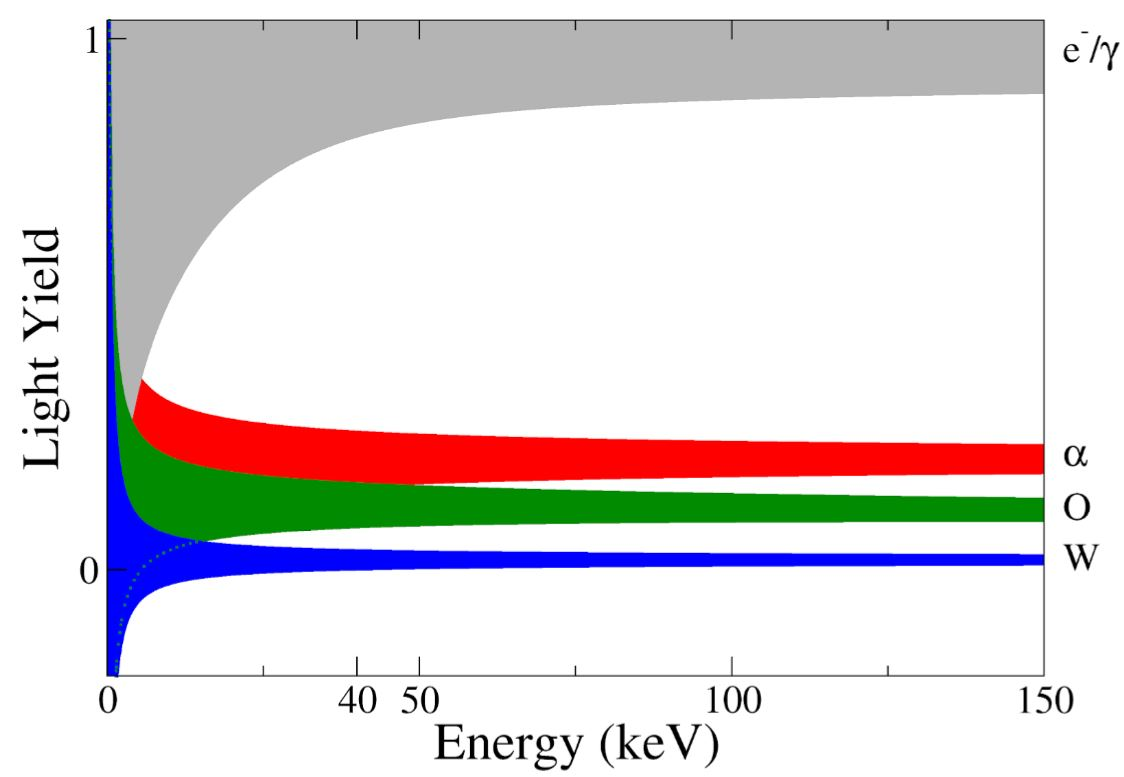
\includegraphics[width=0.85\textwidth]{figures/Bands.JPG}
    \caption{Rappresentazione schematica delle bande di evento nel piano Light Yield in funzione dell'energia per un cristallo di $\text{CaWO}_4$. Si distinguono nettamente la banda grigia superiore dei rinculi elettronici ($e^-/\gamma$) e le bande inferiori associate ai rinculi nucleari di alfa ($\alpha$), ossigeno (O) e tungsteno (W). La larghezza delle bande aumenta a basse energie a causa delle fluttuazioni statistiche nella raccolta dei fotoni. Immagine tratta da \cite{cresst_detectors_2026}.}
    \label{fig:bands}
\end{figure}

Analizzando la Figura~\ref{fig:bands}, è possibile identificare le diverse componenti che popolano il diagramma:
\begin{itemize}
    \item \textbf{Banda $e^-/\gamma$ (regione grigia):} Posizionata attorno a $LY \approx 1$, accoglie i rinculi elettronici derivanti dalla radioattività ambientale $\beta$ e $\gamma$. Rappresenta la quasi totalità del fondo sperimentale.
    \item \textbf{Banda $\alpha$ (regione rossa):} Dovuta a contaminazioni interne o superficiali di emettitori alfa.
    \item \textbf{Bande dei rinculi nucleari (regioni verde e blu):} I nuclei di Ossigeno (O) e Tungsteno (W) mostrano un quenching progressivamente più marcato a causa della loro maggiore massa. Una WIMP di materia oscura, interagendo prevalentemente tramite scattering coerente con i nuclei del bersaglio (con una sezione d'urto che scala come $A^2$, favorendo il Tungsteno pesante), produrrebbe eventi confinati principalmente nella banda del Tungsteno (W) o dell'Ossigeno (O).
\end{itemize}

\section{Scudi attivi e passivi}
\label{sec:scudi}

L'apparato sperimentale di CRESST è protetto da un sistema di schermatura a più livelli, progettato per ridurre al minimo il fondo sperimentale e massimizzare la sensibilità alla materia oscura. Questo sistema si compone di due componenti principali: scudi passivi e scudi attivi.

\begin{itemize}
    \item \textbf{scudi passivi:} materiali ad alta densità come piombo e rame, che circondano il criostato e i moduli rivelatori, assorbendo la radiazione ambientale $\gamma$ e riducendo la radioattività di fondo. Questi strati schermano efficacemente i raggi cosmici e le particelle cariche provenienti dall'ambiente esterno.
    \item \textbf{scudi attivi:} un sistema di scintillatori viene utilizzato per rilevare i muoni cosmici residui ed eliminarli \textit{a posteriori}.
\end{itemize}

In particolare l'articolata successione di scudi passivi, rappresentata in Figura \ref{fig:shielding}, dall'esterno all'interno consta di:

\begin{wrapfigure}{r}{0.45\textwidth}
    \centering
    \vspace{-20pt} % Riduce lo spazio bianco sopra la figura per allinearla al testo
    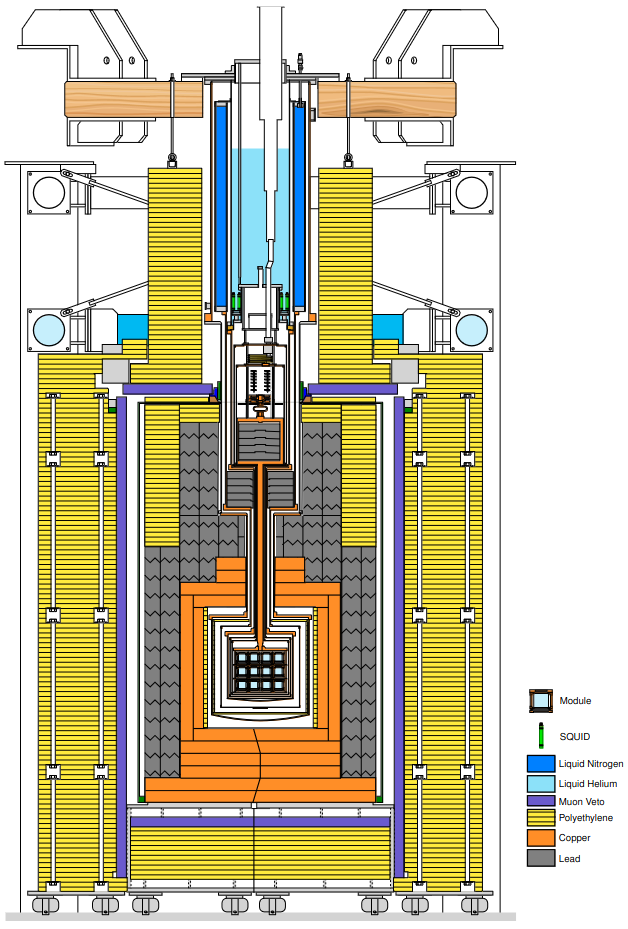
\includegraphics[width=0.42\textwidth]{figures/Schematic-cross-section-of-the-CRESST-setup-27-showing-the-structure-of-the-cryostat.ppm.png}
    \caption{Schema del sistema di schermatura di CRESST.}
    \label{fig:shielding}
    \vspace{-10pt} % Riduce lo spazio bianco sotto la didascalia
\end{wrapfigure}

\begin{enumerate}
    \item uno spesso strato di polietilene (\SI{40}{\cm}), che funge da moderatore per i neutroni ambientali. Grazie alla composizione chimica ricca di idrogeno, il polietilene rallenta i neutroni veloci, riducendo la loro energia fino a valori termici, per poi essere catturati tramite cattura radiativa.
    \item uno strato di piombo di circa \SI{20}{\cm}, che riduce la radioattività ambientale $\gamma$. Poiché il piombo è leggermente radioattivo, a causa della presenza di $^{210}\text{Pb}$, si utilizza piombo o a basso contenuto di questo isotopo, o piombo antico, che ha avuto il tempo di decadere.
    \item uno strato di rame di circa \SI{14}{\cm} estremamente radiopuro, che funge da ultima barriera e riduce al minimo il rumore di fondo.
\end{enumerate}

Inoltre, in Figura \ref{fig:shielding} è rappresentato uno spessore viola associato al termine "muon veto". Questo scudo rappresenta l'ultimo metodo (attivo) di schermaggio contro i muoni cosmici residui. Essendo sotto \SI{1400}{\metre} di roccia, il flusso di muoni cosmici è ridotto di circa sei ordini di grandezza rispetto alla superficie terrestre, raggiungendo un valore di $1$ muone al metro quadro ogni ora, che rischierebbe di contaminare eccessivamente il segnale di materia oscura. 

Per questo motivo viene installato un sistema di scintillatori plastici che, colpiti da un muone, si eccitano, per poi tornare allo stato fondamentale emettendo fotoni di scintillazione, raccolti da tubi fotomoltiplicatori. Quando i fotomoltiplicatori registrano il passaggio di un muone e viene contemporaneamente rilevato un evento nel cristallo, esso viene scartato, poiché non dovuto a materia oscura.
